\documentclass[11pt, a4paper]{article}
\usepackage[margin={3cm, 3cm}]{geometry}

\usepackage[utf8]{inputenc}
\usepackage[swedish]{babel}

\usepackage{parskip}
\usepackage{setspace}
\usepackage[babel]{microtype}
\usepackage[labelsep=period, labelfont=bf, skip=5pt]{caption}
\usepackage{subcaption}
\usepackage{dirtytalk}

\usepackage[style=apa, citestyle=apa]{biblatex}
\addbibresource{bibliography.bib}

\usepackage{amsmath}
\usepackage{amsfonts}
\usepackage{siunitx}

\usepackage{tikz}
\usepackage{svg}
\svgpath{{images/}}
% To include SVG figure:
%\includesvg[inkscapelatex=false, width=\textwidth]{svg_image}

\usepackage{graphicx}
\graphicspath{{images/}}

\title{Magnetisk resonanstomografi}
\author{Björn Sundin\medskip\\\normalsize Fysik 3 - NTI Kronhus}

\begin{document}

\maketitle
\vfill
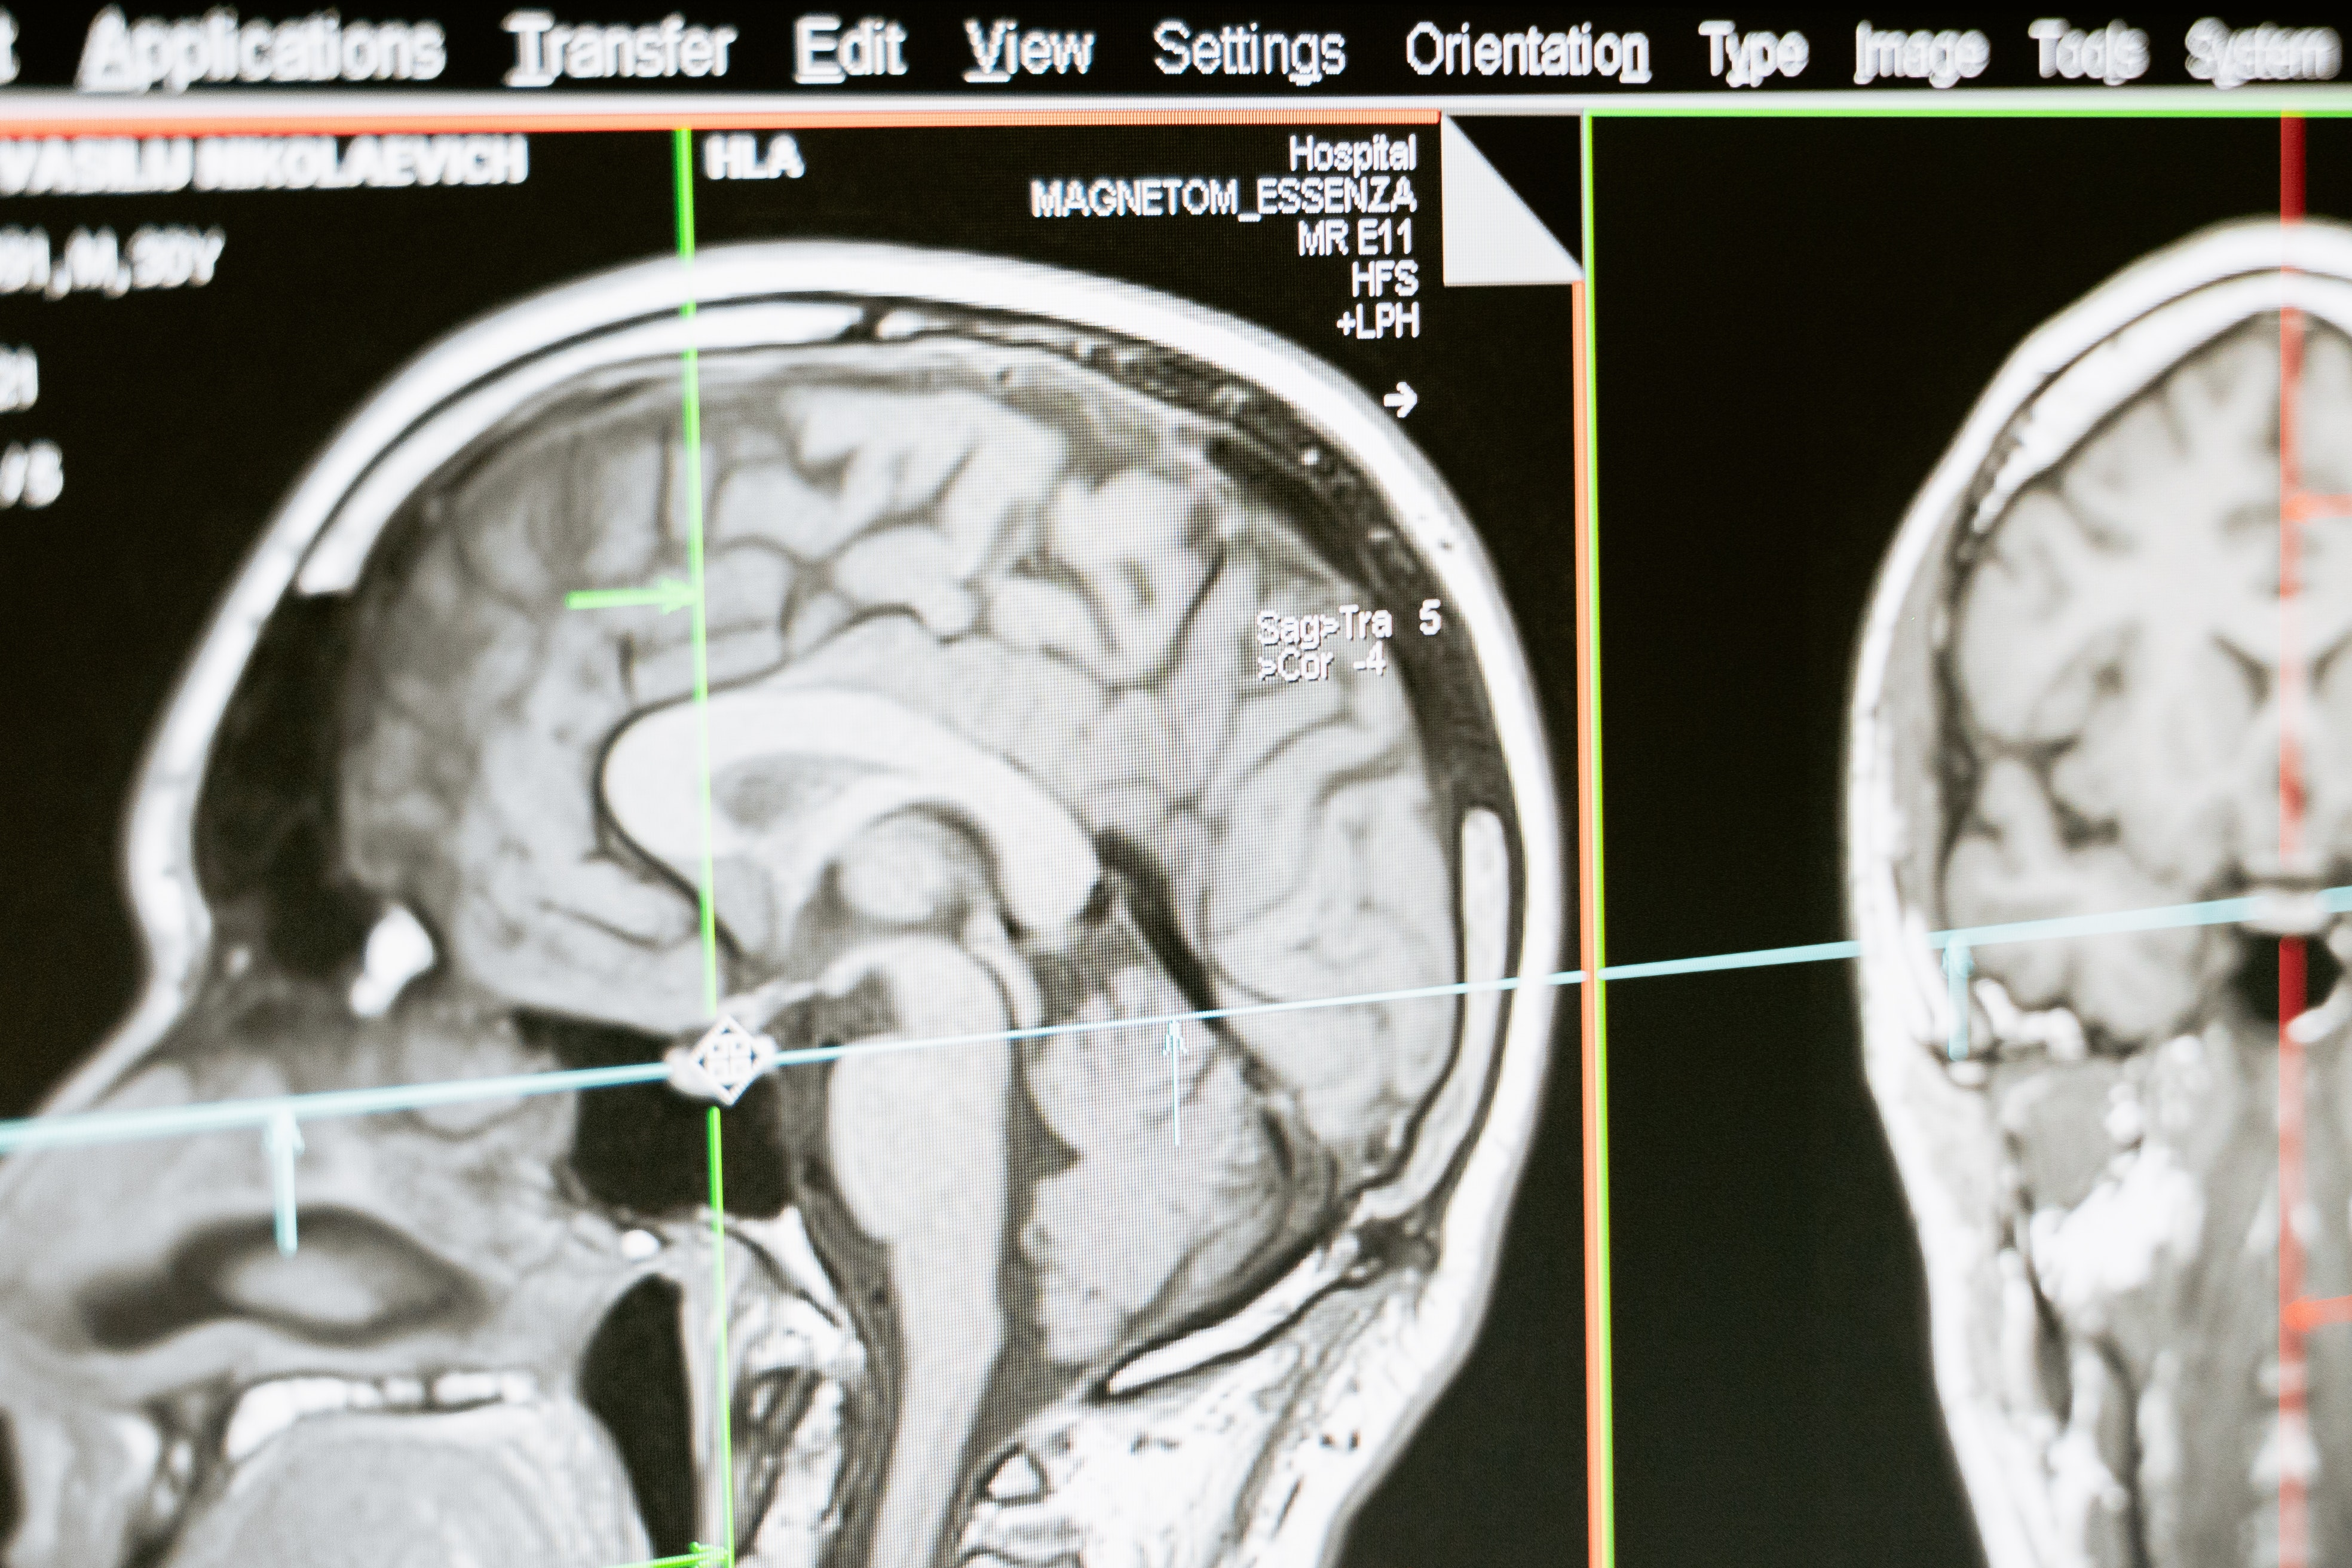
\includegraphics[width=\textwidth]{mri_scan.jpg}
\vspace{1cm}
\vfill

\clearpage
\section{Bakgrund}

Magnetisk resonanstomografi, förkortat MRT eller MRI (Magnetic Resonance Imaging) är en teknik som används inom sjukvården för att skapa detaljrika bilder av vävnad och organ hos människor och djur på ett ofarligt och icke-påträngande sätt \parencite{mri_nobelpris_pressmeddelande}. MRI-scannern som används i sjukvården består av en cylinder med ett skjutbart bord i som patienten ligger på, se figur \ref{fig:mri_patient}. 

Till skillnad från tidigare tekniker för diagnostisk avbildning såsom röntgen, används ingen joniserande strålning i MRI-undersökningar. Istället används ett mycket starkt magnetfält och radiovåg-pulsar. Tekniken bygger på konceptet av kärnmagnetisk resonans/NMR (Nuclear Magnetic Resonance), vars teori hade sina rötter i upptäckten av protonens spinnegenskaper under 1920-talet \parencite{mri_lärobok}.

\begin{figure}[ht]
	\centering
	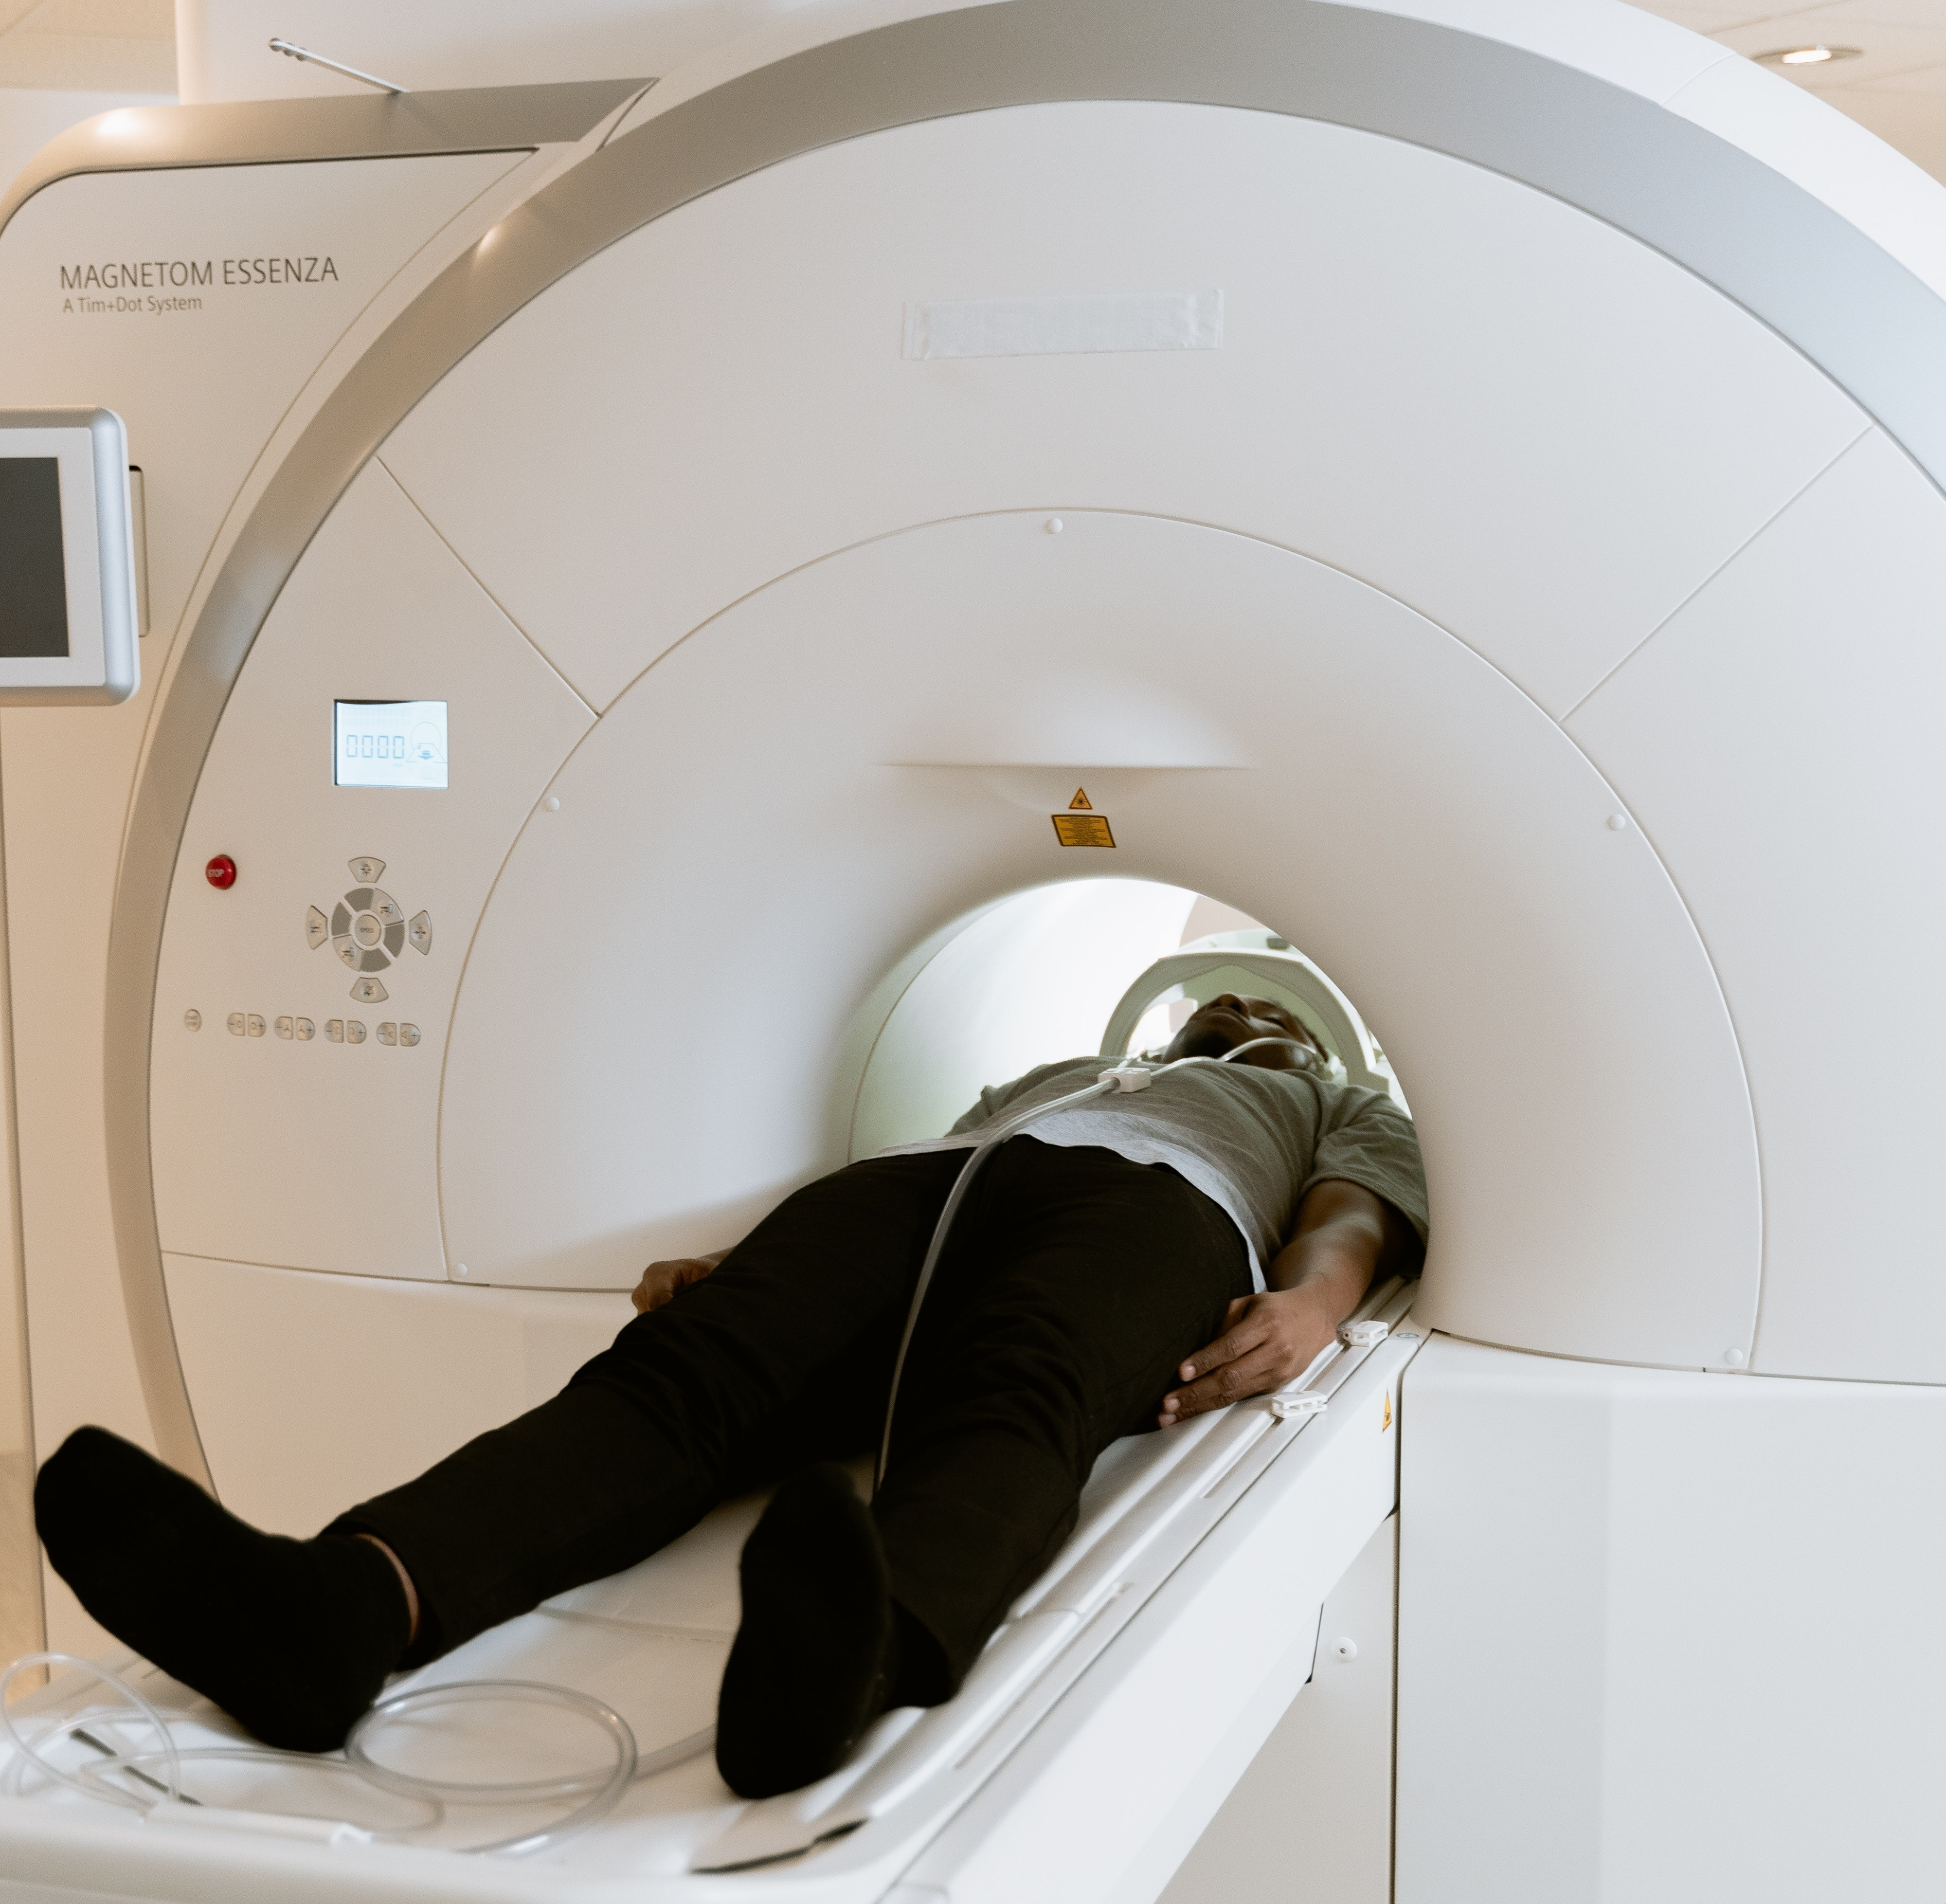
\includegraphics[width=.7\textwidth]{mri_patient}
	\caption{En patient som genomgår en MRI-undersökning. Foto av MART PRODUCTION \parencite*{fig:mri_patient} från Pexels.}
	\label{fig:mri_patient}
\end{figure}

Benämningen NMR används främst för det fysikaliska fenomenet och inte längre i sammanhang av diagnostiska undersökningar av individer \parencite{nmr_eller_mri}. \say{Magnetisk resonans} är mindre specifikt än \say{kärnmagnetisk resonans} eftersom det även finns elektronspinnresonans som involverar elektronen och inte atomkärnan. Ordet \say{nuclear} eller prefixet \say{kärn-} förknippas med farliga saker av allmänheten, så man undviker ofta att använda den mer specifika benämningen trots att det bara syftar på att man studerar atomkärnan.

Kärnmagnetisk resonans används även inom kemin för att undersöka strukturen hos olika ämnen \parencite{nmr_kemi}. Då produceras ett NMR-spektra, istället för en 2D- eller 3D-bild, som avslöjar egenskaper hos ämnet. År 1945 utvecklade Felix Bloch och Edward Mills Purcell, med kunskap om kvantmekaniken som utvecklades under 1930-talet och tidigare, de första mätningarna som använde sig av kärnmagnetisk resonans \parencite{mri_lärobok}. De mätte då signaler från ett vattenprov och ett paraffinprov, och förklarade de experimentella och teoretiska detaljerna av NMR. För detta delade Bloch och Purcell nobelpriset i fysik år 1952 \parencite{nmr_nobelpris}.

Två av de främsta utvecklarna av MRI-teknologin var Paul Lauterbur och Peter Mansfield \parencite{mri_nobelpris_pressmeddelande}. Under 1970-talet gjorde Lauterbur och Mansfield flera upptäckter som lade en grund för utvecklingen av MRI. 1973 beskrev Lauterbur hur gradientmagneter kunde användas tillsammans med NMR för att göra flera endimensionella projektioner av ett objekt, som sedan sätts ihop till en två- eller tre-dimensionell bild. I hans experiment kunde han använda tekniken för att skilja på vanligt och tungt vatten, något som ingen annan avbildningsmetod kunde göra. Samma år utnyttjade Mansfield tillsammans med Peter Grannell gradientmagneter med NMR för att undersöka strukturen i fasta ämnen på ett mer exakt sätt. 1977 tog Mansfield fram en ny metod för NMR-avbildning som utnyttjade egenskaperna hos en effekt som kallas spinn-eko i gradientmagneterna. Denna nya metod kunde producera bilder snabbare än tidigare metoder. Lauterbur och Mansfield fick år 2003 nobelpriset i Fysiologi eller Medicin för sina bidrag till MRI-tekniken \parencite{mri_nobelpris_pressmeddelande}.

Magnetisk resonanstomografi började tillämpas i sjukvården redan i början av 1980-talet, och år 2002 fanns det mer än 22 000 magnetkameror i hela världen \parencite{mri_nobelpris_pressmeddelande}. Utvecklingen av MRI revolutionerade medicinen, och sedan dess har tekniken fortsatt att utvecklas och förfinas \parencite{mri_facts}. Magnetkameran används för att undersöka alla organ i kroppen. Några exempel på problem som undersöks med magnetkameror är abnormaliteter i hjärnan och ryggraden, tumörer och cystor i olika delar av kroppen, bröstcancer, skador i lederna, och hjärtproblem. En annan användning av MRI kallas fMRI (functional Magnetic Resonance Imaging), och innebär att man mäter kognitiv aktivitet i hjärnan genom att undersöka blodflödet i olika delar av hjärnan. Det ger viss information om neuronernas aktivitet även om det inte är vad man direkt mäter.

\clearpage
\section{Utrustning}
Till att börja med kan det vara bra att införa ett koordinatsystem för att benämna olika axlar i MRI-systemet. Riktningen som går från patientens fötter till huvud är Z-axeln. X-axeln går från patientens högra till vänstra sida och Y-axeln går upp från marken, rygg till mage. Det här är ett vanligt koordinatsystem som används inom MRI \parencite{mri_for_radiologists}.

\begin{figure}[hp]
	\centering
	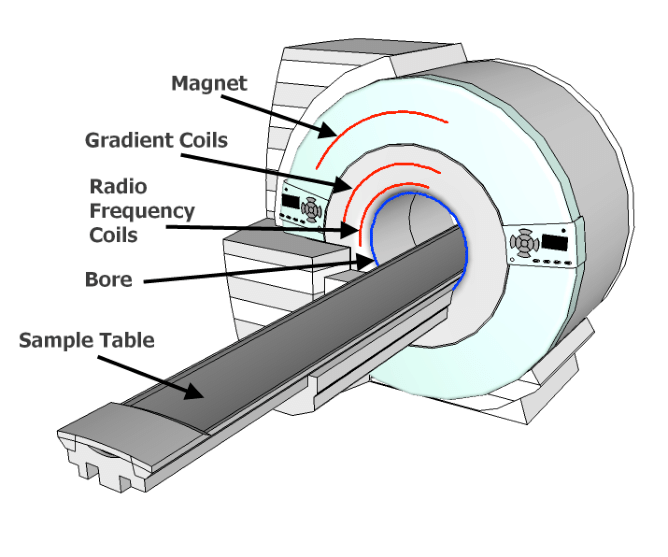
\includegraphics[width=.8\textwidth]{mri_schematic}
	\caption{Diagram av en magnetkamera och placeringen av de olika spolarna. Bildkälla: \cite{fig:mri_spolar_diagram}.}
	\label{fig:mri_diagram}
\end{figure}

Figur \ref{fig:mri_diagram} visar ett diagram av de primära komponenterna i en magnetkamera. Magnetkamerans största beståndsdel är den mycket starka elektromagneten, placerad längst ut från cylinderns center. Elektromagneten består av en solenoidspole som bildar ett magnetiskt fält med flödestätheten $B_0$ i centret där patienten befinner sig under undersökningen. $B_0$ brukar vara 1.5 T eller 3 T för kliniskt bruk \parencite{understanding_mri}. Figur \ref{fig:solenoid} visar en sådan spole, där de raka linjerna motsvarar fältet $B_0$ som går längs Z-axeln i MRI-systemet. För att uppnå den höga fältstyrkan på ett effektivt sätt används en supraledande metallegering i spolen, som kyls ner till runt 4 K med hjälp av flytande helium. Det gör att strömmen kan flöda med minimal resistans och därmed att den magnetiska flödestätheten blir större för samma effekt, enligt $B_0\propto\sqrt\frac{P}{R}$. Resistansen i supraledaren är dock så låg att detta samband inte beskriver systemet korrekt. Magneten kan hålla kvar strömmen helt utan pålagd spänning i flera år efter en första upprampning \parencite{mri_for_radiologists}.

\begin{figure}[ht]
	\centering
	\includesvg{Solenoidspole}
	\caption{En solenoidspole som kan liknas med den starka elektromagneten i MRI-systemet. Bilkälla: \cite{fig:solenoid}.}
	\label{fig:solenoid}
\end{figure}

Närmare centret av magnetkamerans cylinder finns tre gradient\-magnet-spolar (se figur \ref{fig:mri_diagram}) \parencite{understanding_mri}. Dessa har syftet att variera magnetfältet linjärt över valfri tredimensionell riktning. Gradientmagneterna motsvarar de tre axlarna och deras styrkor kan justeras dynamiskt för att ändra det resulterande fältets riktning. Eftersom endast en tredimensionell relativ lutning av fältstyrka behövs är gradientmagneterna relativt svaga och är inte nedkylda. Gradientmagneterna justerar bara riktningen av det starka magnetfältet som kommer från den primära elektromagneten.

Den tredje uppsättningen spolar är RF(Radio Frequency/radiofrekvens)-spolarna, som ligger ännu närmare patienten. Syftet med dessa är att skicka energi i form av elektromagnetiska vågor med en viss (icke-joniserande) frekvens i MHz-området (radiovågor) in i vävnaden, samt att detektera emitterade radiovågor från vävnaden. Radiofrekvens-fältet benämns $B_1$. För fMRI används en separat RF-spole vid huvudet för att maximera signalerna från hjärnan. Eftersom det finns många andra källor av radiovågor (exampelvis från radio\-kommunikation) som når ut till där magnetkameran befinner sig, behöver rummet vara en faradays bur. På så sätt kontaminerar inte de yttre och de inre radiovågorna varandra.

En annan mycket viktig komponent av MRI-systemet är datorerna som behandlar all data och som ger operatören ett grafiskt användargränssnitt att styra med och se resultaten på. Dessa är placerade i ett annat rum, kontrollcentret där operatören sitter. Datan som samlas in av magnetkameran transformeras med komplexa signalbehandlings-algoritmer för att producera de resulterande bilderna.

\clearpage
\section{Teori}

%En grundläggande princip som utnyttjas i denna teknik är att energin som detekteras i NMR är proportionell mot magnetfältets styrka. Gradientmagneterna gör att magnetfältets styrka varierar linjärt på en axel, och detta gör alltså att den endimensionella projektionen kan erhållas. 

I magnetisk resonanstomografi studeras kärnan hos väte, protonen. Detta är delvis för att människor innehåller så mycket väte, främst i vattnet som vi består av till runt 66\% \parencite{mri_nobelpris_pressmeddelande}. Men det är också på grund av protonens kvantmekaniska egenskaper. Härefter kommer en bakgrund till de kvantmekaniska principerna som MRI bygger på.

Subatomära partiklar har en kvantmekanisk egenskap som kallas spinn \parencite{college_physics}. Spinnkvanttalet $s$ bestämmer magnituden av ett inre rörelsemängdsmoment $\vec{S}$ som är speciellt för varje typ av partikel. Man kan tänka sig att partikeln roterar runt en egen axel på samma sätt som en boll kan göra i klassisk fysik. Den liknelsen håller dock inte hela vägen, och den är extra orimlig för just elektroner - den hypotetiska ytan hade behövt röra sig med en hastighet snabbare än ljusets för att det inre rörelsemängdsmomentet ska vara korrekt \parencite{electron_spin}. 

\say{spinn} används här som synonym till $\vec{S}$, alltså \say{inre rörelsemängds\-moment hos en subatomär partikel}, och är en vektor. I klassisk fysik bestäms rörelse\-mängdsmomentet hos en partikel av kryssprodukten $\vec{L}=m\vec{r}\times\vec{v}$, där $\vec{r}$ är partikelns position relativt rotationens center och $\vec{v}$ är hastighetsvektorn vid samma tidpunkt. Man kan tänka sig att vår subatomära partikel består av mindre partiklar, och det totala rörelsemängdsmomentet hos dessa har samma riktning som spinnet. Alltså uppåt om den roterar motsols i planet sett uppifrån. Magnituden av spinnet bestäms av $S=\hbar\sqrt{s(s+1)}\:\left[\si{kg.m^2.s^{-1}}\right]$ (där $\hbar=\frac{h}{2\pi}$) \parencite{college_physics}. $s$ förekommer kvantiserat i steg av $\frac{1}{2}$ hos olika partiklar, vilket innebär att $S$ och $\vec{S}$ också är kvantiserat. Protoner, neutroner och elektroner har $s=\frac{1}{2}$ medan vissa andra partiklar har $s=1$ eller $s=0$. Partiklar med heltals-spinn (inklusive 0) klassas som fermioner och partiklar med halvtaligt spinn är bosoner \parencite{subatomic_particles}.

Partiklar som både har en laddning och ett spinntal $s\neq 0$ beter sig som en magnet, med ett magnetiskt dipolmoment $\vec{\mu}$ riktat i samma riktning som $\vec{S}$ om laddningen är positiv. Detta kan liknas med en elektromagnet, där negativt laddade elektroner flödar i en cirkulär rörelse och därmed bildar ett magnetiskt dipolmoment med motsatta riktningen av elektronens rörelsemängdsmoment. Dipolmomentets magnitud definieras klassiskt som strömmen i spolen gånger cirkelns area, $\mu=IA=\pi Ir^2$, och har enheten \si{\left[A.m^2\right]} \parencite{magnetism}. Dipolmomentet hos en subatomär partikel relateras till spinnet genom $\vec{\mu}=\gamma\vec{S}$, där $\gamma$ är den gyromagnetiska kvoten för partikeln \parencite{larmor_precession}, som vi återkommer till. $\gamma$ är \SI{2.675 221 900(18) e8}{\left[s^{-1}.T^{-1}\right]} för protoner \parencite{gyro_ratio}. 

\begin{figure}[p]
	\centering
	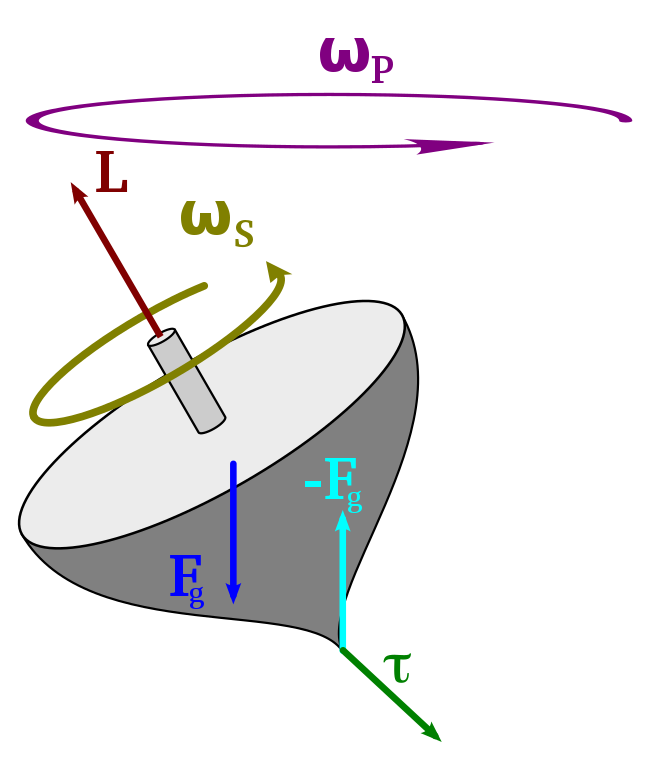
\includegraphics[width=.5\textwidth]{snurra_precession}
	\caption{Precession av en snurra, där $L$ är rörelsemängdsmoment-vektorn, $\omega_p$ är precessions-frekvensen och $\omega_s$ är spinnfrekvensen. Vridmomentet $\tau$ bildas av gravitationskraften $F_g$ och den reaktiva normalkraften $-F_g$ vid bordets yta. Riktningen av detta vridmoment vrids på grund av det egna spinnet och gör att snurran precesserar. Bildkälla: Xavier Snelgrove \parencite*{fig:snurra_precession}, CC BY-SA 2.5, via Wikimedia Commons.}
	\label{fig:snurra_precession}
\end{figure}
\begin{figure}[p]
	\centering
	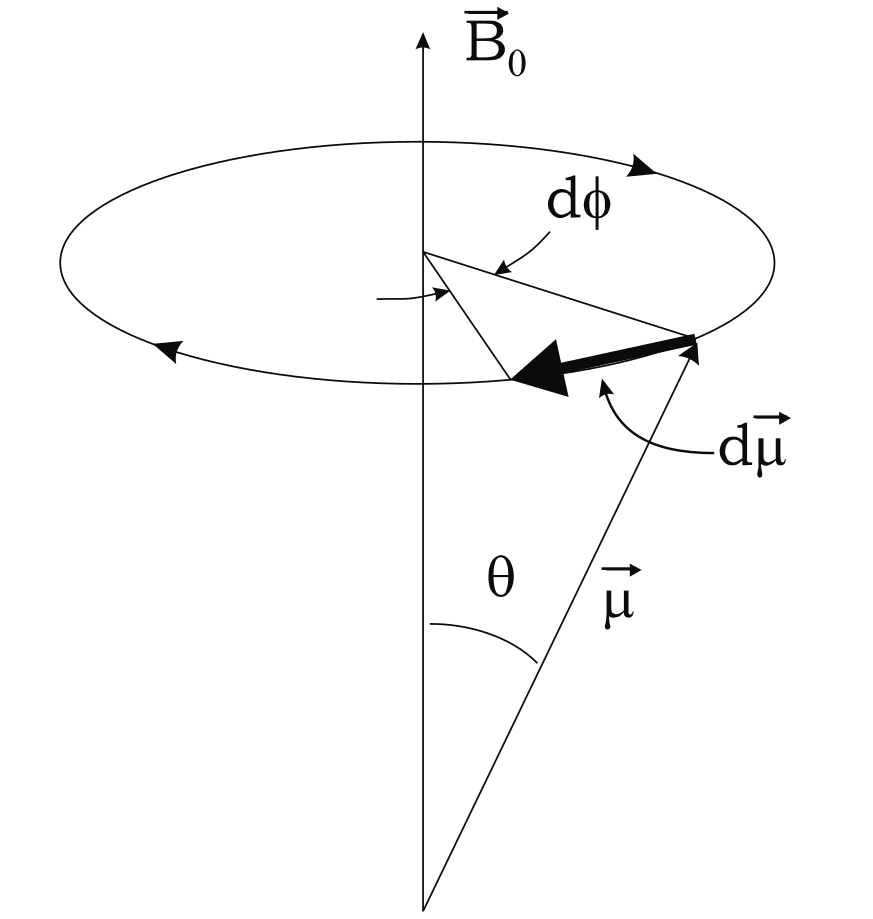
\includegraphics[width=.5\textwidth]{magnetic_moment_precession}
	\caption{En partikel med ett kvantspinn som gör att det magnetiska dipolmomentet $\vec\mu$ bildas, placerat i ett yttre magnetfält $\vec B_0$ som gör att dipolmomentet precesserar likt snurran. Källa: \cite{mri_lärobok}}
	\label{fig:magnetiskt_moment_precession}
\end{figure}

När en partikel med en egen magnetisk dipol dessutom placeras i ett homogent yttre magnetfält $\vec{B_0}$ så börjar dipolmomentet precessera runt det likt hur en makroskopisk snurra precesserar runt ett gravitationsfält \parencite{larmor_precession}, se figur \ref{fig:snurra_precession} och \ref{fig:magnetiskt_moment_precession}. Detta leder till två saker:
\begin{itemize}
	\item Spinnet $\vec{S}$ har en viss vinkel ($\theta$ i figur \ref{fig:magnetiskt_moment_precession}) mot Z-axeln. Projektionen av $\vec{S}$ längs Z-axeln bestäms av $S_z=m_s\hbar$, där $m_s$ är kvanttalet för spinnets projektion och är kvantiserat till värdena $m_s=s+n$ där $n\in\{-2s..0\}$ \parencite{university_physics}.
	\item $\vec{\mu}$ precesserar med en viss frekvens som kallas Larmorfrekvensen, och även denna bestäms med hjälp av den gyromagnetiska kvoten i Larmor-ekvationen \parencite{mri_lärobok}:
	\begin{equation}\label{eq:larmor}
		\omega=2\pi f=\gamma B_0\:[\si{rad/s}]
	\end{equation}
	Frekvensen ökar alltså linjärt med magnetfältetets styrka.
\end{itemize}

Hos protonen, likt elektronen, är $s=\frac{1}{2}$ och $m_s=\pm\frac{1}{2}$ \parencite{college_physics}. Vinkeln av spinnet mot Z-axeln blir då $\theta_z=\arccos\sqrt\frac{1}{3}\approx54.7^\circ$. Eftersom $s$ alltid har samma värde för elektroner brukar spinnkvanttalet utelämnas från kvanttalen, eller syfta på $m_s$. $m_s=\frac{1}{2}$ innebär att $\vec{\mu}$ precesserar parallellt med $\vec{B_0}$ och $m_s=-\frac{1}{2}$ innebär att det precesserar antiparallellt mot fältet. Det parallella tillståndet har något lägre potentiell energi än det antiparallella tillståndet eftersom det tar ett arbete för att motverka magnetfältet \parencite{electron_spin}. Spinnprojektionstalet $m_s$ kan ändras hos en partikel eftersom det motsvarar olika energinivåer, medan magnituden $s$ är konstant. 

Tillbaka till magnetkameran. Vi börjar med att bortse från gradientmagneterna. När en människa placeras i magnetkameran utsätts alla protonerna i kroppen för det magnetiska fältet $\vec{B_0}$ riktat från fötterna till huvudet på personen \parencite{understanding_mri}. Det gör att ungefär hälften av protonernas magnetiska moment precesserar i samma riktning som magnetfältet och hälften antiparallellt. Eftersom de antiparallella har en något högre energinivå kommer det dock finnas ett litet underskott av dessa. För 1 miljon protoner som precesserar antiparallellt finns det ungefär 10-20 stycken fler\footnote{Från egna beräkningar. Siffran i artikeln av \textcite{understanding_mri} är tagen från boken \citetitle{mri_made_easy} av \textcite{mri_made_easy}, och är inte helt rimlig för parametrarna i en magnetkamera.} som precesserar parallellt med $\vec{B_0}$. Protonerna precesserar med (nästan) samma frekvenser, men eftersom de har slumpmässig fasförskjutning kommer det totala magnetiska dipolmomentet $\vec{M}$ i personen vara riktat i precis samma riktning som $\vec{B_0}$, vilket illustreras i figur \ref{fig:spinn_vektorer}. Personens totala magnetisering i detta tillfälle kallas också för den longitudinella magnetiseringen.

\begin{figure}[ht]
	\centering
	\includesvg[width=0.67\textwidth]{spinn_vektorer}
	\caption{Illustrativt diagram av det magnetiska momentet hos olika protoner i kroppen av personen i magnetkameran. Vinklarna är skalenliga men inte längderna eller antalen. Rosa vektorer är individuella $\vec{\mu}$ hos olika protoner vid en viss tidpunkt, med något fler i parallellt spinntillstånd än antiparallellt. Blå vektor är hela personens magnetiska moment $\vec{M}=\sum{\vec{\mu_n}}$ (longitudinell magnetisering) och har därmed samma riktning som $\vec{B_0}$. Figuren är originell.}
	\label{fig:spinn_vektorer}
\end{figure}

$\vec{M}$ kan inte mätas eftersom den ligger i riktning med $\vec{B_0}$ \parencite{understanding_mri}. För att få information om vävnaden och dess struktur använder man sig av de tidigare nämnda RF-spolarna. Strömmen i en RF-spole varierar med en frekvens vilket gör att magnetfältet som bildas av spolen oscillerar med den frekvensen; elektromagnetiska vågor sänds ut \parencite{mri_for_radiologists}. När frekvensen är inställd till Larmorfrekvensen, alltså den som protonernas egna magnetfält precesserar med, så sker magnetisk resonans. Det innebär två saker \parencite{understanding_mri}:
\begin{itemize}
	\item Protoner kan ta upp energin $\Delta E=hf=\hbar\gamma B_0$ (ekvation \ref{eq:larmor}) och gå från det parallella spinntillståndet till det antiparallella tillståndet.
	\item Alla protonernas magnetiska moment börjar precessera i fas med varandra och de elektromagnetiska vågorna, så att $\vec{M}$ precesserar på samma sätt som en enskild proton.
\end{itemize}

Förresten, varför är inte alla protoner i det parallella tillståndet om det har en lägre energinivå? Om protonen betedde sig som en vanlig magnet hade ju alla lagt sig i riktning med magnetfältet. Eftersom vi nu vet energiskillnaden mellan de två spinntillstånden kan vi förklara varför det alltid är just den andelen parallella och antiparallella protoner, med hjälp av Boltzmannfaktorn \parencite[s. 90]{mri_lärobok}:
\begin{equation}
	\frac{n_d}{n_u}=e^\frac{-\Delta E}{kT}=e^\frac{-\hbar\gamma B_0}{kT}
\end{equation}
Där $n_d$ är antalet protoner i det antiparallella spinntillståndet och $n_u$ är antalet i det parallella tillståndet. $k$ är Boltzmanns konstant och T är temperaturen. Ekvationen anger alltså relationen mellan sannolikheten av tillståndet med högre energi och sannolikheten av tillståndet med lägre energi, som en funktion av temperaturen och skillnaden i energi mellan de två tillstånden. För $T=\SI{310}{K}$ (kroppstemperatur), $B_0=\SI{1.5}{T}$, och $n_d=\SI{1000000}{}$ ger detta att $n_u\approx\SI{1000010}{}$ protoner. Orsaken är alltså delvis att energiskillnaden mellan tillstånden är så liten (\SI{5.3e-7}{eV}). Om det var normala magneter hade skillnaden i potentiell energi mellan de två riktningarna varit mer än enorm i jämförelse. Om temperaturen i personen vore väldigt nära den absoluta nollpunkten skulle andelen protoner i den högre energinivån också varit lägre.

Hur många av protonerna som övergår till det antiparallella tillståndet på grund av radiovåg-pulsen beror på styrkan och varaktigheten av den \parencite{mri_for_radiologists}. Det innebär att vinkeln mot Z-axeln $\theta_z$ av $\vec{M}$ går från $0^\circ$ till en ny vinkel som är större ju fler protoner som tagit upp energi från pulsen. Här betraktar vi en RF-puls som gör att $\vec{M}$ ligger i XY-planet precis när pulsen stängs av, en så kallad $90^\circ$-puls. Andra pulsar används också, exempelvis $180^\circ$-pulsar där den resulterande magnetiseringen precesserar antiparallellt.

När pulsen är avslagen börjar protonerna frigöra överskottsenergin och därmed återgå till sina ursprungliga energinivåer \parencite{understanding_mri}. På samma gång hamnar protonernas dipolmoment återigen ur fas med varandra. Denna process kallas relaxation och sker över tid så att $\vec{M}$ rör sig på ett sätt som illustreras i figur \ref{fig:relaxation}. Eftersom $\vec{M}$ nu varierar gör det att det magnetiska flödet i RF-spolarna också varierar, och en spänning induceras enligt $U=-N\frac{\mathrm{d}\Phi}{\mathrm{d}t}$ där $N$ är antalet varv i spolen och $\Phi$ är det magnetiska flödet (faradays induktionslag). På så sätt kan nu systemet känna av en MR-signal.

\begin{figure}[ht]
	\centering
	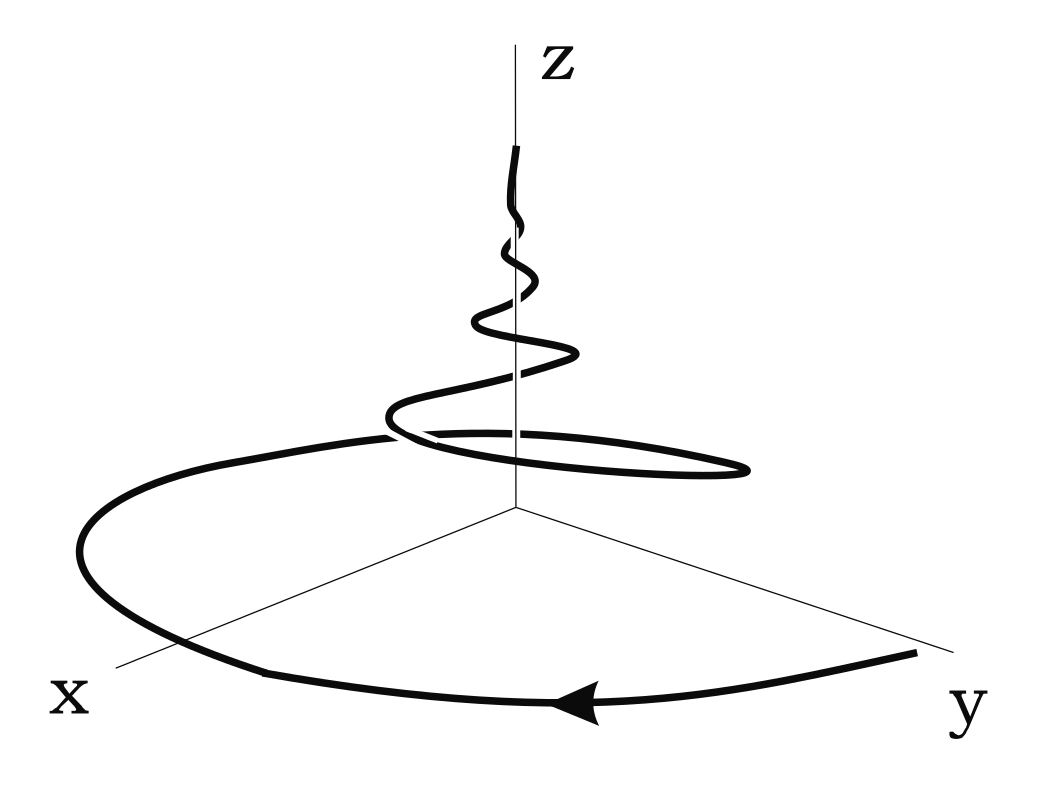
\includegraphics[width=0.7\textwidth]{relaxation}
	\caption{Rörelsen av $\vec{M}$ under relaxationen efter en $90^\circ$-RF-puls. Källa: \cite{mri_lärobok}.}
	\label{fig:relaxation}
\end{figure}

Relaxationen delas upp i två delar som orskas av olika processer, benämnda T1 och T2 \parencite{understanding_mri}. T1-relaxation syftar på återställningen av den longitudinella magnetiseringen, alltså hur projektionen av $\vec{M}$ på Z-axeln, $M_z$, förändras över tid direkt efter RF-pulsen. T1-relaxationen beror bara på att en mycket liten andel protoner återgår till sin lägre energinivå där de precesserar parallellt med $\vec{B_0}$ istället för antiparallellt. T1-relaxationens graf är en exponentiellt avtagande funktion som går från $0$ till den ursprungliga longitudinella magnetiseringen $M_{z0}$. T1-tiden bestämmer hur lång tid relaxationen tar. Eftersom det inte går att säga exakt när den är färdig bestämmer T1-tiden hur lång tid det tar för $M_z$ att gå från 0 till $1-\frac{1}{e}\approx63\%$ av sitt slutliga värde. Personens totala magnetiska dipolmoment i Z-led efter RF-pulsen kan alltså beskrivas av funktionen \parencite{t1_relaxation}: 
\begin{equation}
	M_z(t)=M_{z0}(1-e^{-\frac{t}{T_1}})	
\end{equation}
T1-tiden beror på flödestätheten $B_0$ samt hur snabbt molekylerna runt protonen rör sig. Molekylernas rörelse genererar varierande magnetfält som påverkar protonen \parencite{understanding_mri}. Om molekylerna rör sig med frekvenser nära protonens Larmorfrekvens är T1-tiden kortare eftersom det leder till att protonen mer effektivt ger bort energi. Eftersom Larmorfrekvensen ökar linjärt med $B_0$ påverkar även magnetfältets styrka T1-tiden. Generellt ger en starkare magnet en längre T1-tid \parencite{t1_relaxation}. Olika molekyler har olika rörelsefrekvens och därmed är T1-tiden olika för olika ämnen i kroppen \parencite{understanding_mri}. Till exempel är T1 för obundet vatten längre än för delvis bundet vatten. Fett brukar ha en kort T1-tid.

T2-relaxationen orsakas endast av att precessionen av protonerna hamnar ur fas med varandra igen efter resonansen \parencite{understanding_mri}. Det finns två orsaker till detta:
\begin{enumerate}
	\item Protonernas egna magnetfält påverkar varandra och orsakar små variationer i Larmorfrekvensen hos individuella protoner enligt ekvation (\ref{eq:larmor}). Svängningar med olika frekvens hamnar ur fas över tid.
	\item Om $B_0$-fältet inte är helt homogent så leder även det till att protonerna får små skillnader i Larmorfrekvens. Eftersom det är en konstant effekt är det möjligt att motverka den till en viss grad.
\end{enumerate}

\clearpage
\section{Fördelar och nackdelar}


\clearpage
\section{Avslutning}

\clearpage
\printbibliography

\end{document}
